\textbf{Phần 1. Trắc nghiệm lựa chọn (Học sinh quan sát hình và chọn đáp án đúng)}
\setcounterpageref{ex}{0}

% --- CÂU 1 ---
\begin{ex} %[1D1N02]
Đếm số chấm tròn trong khung dưới đây và cho biết số mười được viết bằng chữ số nào?
\begin{center}
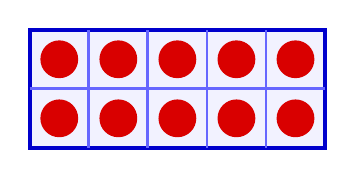
\begin{tikzpicture}[scale=0.75, baseline=(current bounding box.center)]
  % Khung 10 ô (2 hàng 5 cột)
  \draw[line width=1.5pt, blue!80!black, fill=blue!5] (0,0) rectangle (5,2);
  \draw[line width=1pt, blue!60] (0,1) -- (5,1);
  \foreach \x in {1,2,3,4} {
    \draw[line width=1pt, blue!60] (\x,0) -- (\x,2);
  }
  % 10 chấm tròn đỏ
  \foreach \x in {0.5, 1.5, 2.5, 3.5, 4.5} {
    \fill[red!85!black] (\x, 1.5) circle (0.32cm);
    \fill[red!85!black] (\x, 0.5) circle (0.32cm);
  }
\end{tikzpicture}
\end{center}
\choice
{\True $10$}
{$1$}
{$01$}
{$100$}
\loigiai{
Trong khung có đúng $10$ chấm tròn đỏ.\\
Số mười được viết bằng chữ số là $10$.\\
\textbf{Đáp án của câu hỏi là A}
}
\end{ex}

% --- CÂU 2 ---
\begin{ex} %[1D1N02]
Chú chim nhỏ đang đậu ở cành số $6$, cành cây liền sau mang số mấy?
\begin{center}
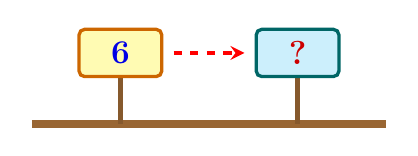
\begin{tikzpicture}[scale=0.75, baseline=(current bounding box.center)]
  \draw[line width=3pt, brown!80!black] (-3,0) -- (3,0);
  % 2 cành rẽ nhánh
  \draw[line width=2pt, brown!70!black] (-1.5,0) -- (-1.5,1.2);
  \draw[line width=2pt, brown!70!black] (1.5,0) -- (1.5,1.2);
  % Biển số
  \draw[fill=yellow!30, draw=orange!80!black, line width=1.2pt, rounded corners=2pt] (-2.2,0.8) rectangle (-0.8,1.6);
  \node[font=\large\bfseries, text=blue!90!black] at (-1.5,1.2) {6};
  \draw[fill=cyan!20, draw=teal!80!black, line width=1.2pt, rounded corners=2pt] (0.8,0.8) rectangle (2.2,1.6);
  \node[font=\large\bfseries, text=red!80!black] at (1.5,1.2) {?};
  \draw[->, >=stealth, dashed, line width=1.2pt, red] (-0.6,1.2) -- (0.6,1.2);
\end{tikzpicture}
\end{center}
\choice
{$5$}
{$8$}
{\True $7$}
{$9$}
\loigiai{
Đếm số liên tiếp: $6, 7, 8, \dots$\\
Số đứng liền sau của số $6$ là số $7$.\\
\textbf{Đáp án của câu hỏi là C}
}
\end{ex}

% --- CÂU 3 ---
\begin{ex} %[1D1H02]
Đoàn tàu chở các số từ $6$ đến $10$. Toa tàu đứng liền trước số $10$ mang số mấy?
\begin{center}
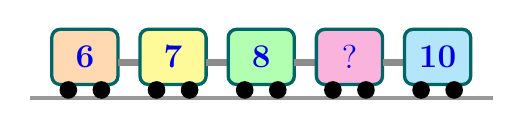
\begin{tikzpicture}[scale=0.7, baseline=(current bounding box.center)]
  \draw[line width=1.5pt, gray!80] (-4.2,-0.55) -- (4.2,-0.55);
  % 5 toa
  \foreach \i/\num/\cl in {0/6/orange!30, 1/7/yellow!40, 2/8/green!30, 3/{$\mathbf{?}$}/magenta!30, 4/10/cyan!30} {
    \draw[fill=\cl, draw=teal!80!black, line width=1.2pt, rounded corners=3pt] (-3.8+\i*1.6,-0.3) rectangle (-2.6+\i*1.6,0.7);
    \node[font=\large\bfseries, text=blue!90!black] at (-3.2+\i*1.6, 0.2) {\num};
    \fill[black] (-3.5+\i*1.6,-0.4) circle (0.16);
    \fill[black] (-2.9+\i*1.6,-0.4) circle (0.16);
    \ifnum\i<4
      \draw[line width=2.5pt, gray!90] (-2.6+\i*1.6,0.1) -- (-2.2+\i*1.6,0.1);
    \fi
  }
\end{tikzpicture}
\end{center}
\choice
{$8$}
{\True $9$}
{$7$}
{$6$}
\loigiai{
Thứ tự các số: $6, 7, 8, 9, 10$.\\
Số đứng liền trước số $10$ là số $9$.\\
\textbf{Đáp án của câu hỏi là B}
}
\end{ex}

% --- CÂU 4 ---
\begin{ex} %[1D1H02]
Ba bạn gấu cầm các quả bóng bay mang số $7$, $\mathbf{?}$, $9$. Quả bóng bay ở giữa mang số nào?
\begin{center}
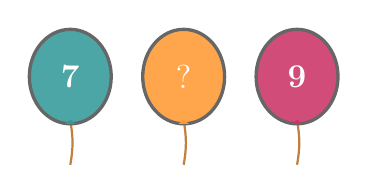
\begin{tikzpicture}[scale=0.8, baseline=(current bounding box.center)]
  \foreach \x/\num/\c in {-1.8/7/teal, 0/{$\mathbf{?}$}/orange, 1.8/9/purple} {
    \draw[line width=0.8pt, brown] (\x,-0.9) to[out=80,in=-80] (\x,-0.2);
    \draw[fill=\c!70, draw=black!60, line width=1.2pt] (\x,0.5) ellipse (0.65cm and 0.75cm);
    \fill[\c!80] (\x-0.08,-0.25) -- (\x+0.08,-0.25) -- (\x,-0.18) -- cycle;
    \node[font=\large\bfseries, text=white] at (\x,0.5) {\num};
  }
\end{tikzpicture}
\end{center}
\choice
{$6$}
{$10$}
{$5$}
{\True $8$}
\loigiai{
Số đứng ở giữa số $7$ và số $9$ là số $8$.\\
\textbf{Đáp án của câu hỏi là D}
}
\end{ex}

% --- CÂU 5 ---
\begin{ex} %[1D1H02]
Đếm ngược từ $10$ về $6$ trên thân chú sâu: $10, 9, 8, \dots, 6$. Đốt thân có dấu $\mathbf{?}$ là số mấy?
\begin{center}
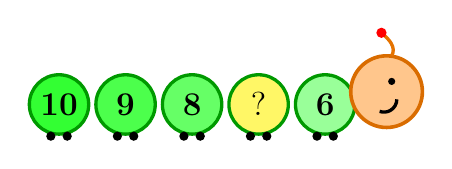
\begin{tikzpicture}[scale=0.65, baseline=(current bounding box.center)]
  \foreach \x/\num/\c in {0/10/green!80, 1.3/9/green!70, 2.6/8/green!60, 3.9/{$\mathbf{?}$}/yellow!60, 5.2/6/green!40} {
    \draw[fill=\c, draw=green!60!black, line width=1.2pt] (\x,0) circle (0.58cm);
    \node[font=\large\bfseries, text=black] at (\x,0) {\num};
    \fill[black] (\x-0.16,-0.62) circle (0.09); \fill[black] (\x+0.16,-0.62) circle (0.09);
  }
  % Đầu sâu
  \draw[fill=orange!45, draw=orange!85!black, line width=1.3pt] (6.4,0.25) circle (0.7cm);
  \fill[black] (6.5,0.45) circle (0.07);
  \draw[line width=1.2pt] (6.6,0.1) arc (0:-110:0.25);
  \draw[line width=1.2pt, orange!90!black] (6.5,0.95) to[out=60,in=-40] (6.3,1.4);
  \fill[red] (6.3,1.4) circle (0.1);
\end{tikzpicture}
\end{center}
\choice
{$6$}
{$8$}
{$9$}
{\True $7$}
\loigiai{
Đếm lùi từ 10 về 6: $10, 9, 8, 7, 6$.\\
Số còn thiếu là số $7$.\\
\textbf{Đáp án của câu hỏi là D}
}
\end{ex}

% --- CÂU 6 ---
\begin{ex} %[1D1H02]
Trong các thẻ số dưới đây, thẻ nào mang số gồm \textbf{hai chữ số}?
\begin{center}
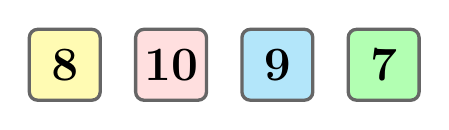
\begin{tikzpicture}[scale=0.75, baseline=(current bounding box.center)]
  \foreach \i/\num/\c in {0/8/yellow!30, 1/10/pink!50, 2/9/cyan!30, 3/7/green!30} {
    \draw[fill=\c, draw=black!60, line width=1.2pt, rounded corners=3pt] (\i*1.8,-0.4) rectangle (\i*1.8+1.2,0.8);
    \node[font=\LARGE\bfseries, text=black] at (\i*1.8+0.6, 0.2) {\num};
  }
\end{tikzpicture}
\end{center}
\choice
{\True $10$}
{$8$}
{$9$}
{$7$}
\loigiai{
Số $10$ được ghép từ hai chữ số: chữ số $1$ và chữ số $0$.\\
Các số $7, 8, 9$ chỉ có một chữ số.\\
\textbf{Đáp án của câu hỏi là A}
}
\end{ex}

% --- CÂU 7 ---
\begin{ex} %[1D1V02]
Hai bàn tay xòe ra dưới đây có tất cả bao nhiêu ngón tay?
\begin{center}
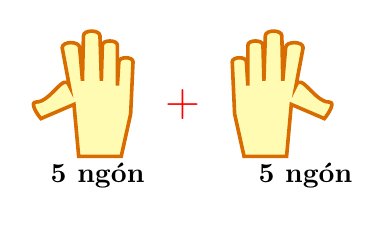
\begin{tikzpicture}[scale=0.6, baseline=(current bounding box.center)]
  % Bàn tay trái
  \begin{scope}[shift={(-2.2,0)}]
    \draw[fill=yellow!30, draw=orange!85!black, line width=1.3pt]
      (0,-0.6) -- (-0.1,0.5) -- (-0.8,0.2) to[out=130,in=180] (-0.9,0.55) to[out=0,in=110] (-0.2,0.9)
      -- (-0.35,1.7) to[out=90,in=90] (0.02,1.7) -- (0.08,1.0)
      -- (0.1,1.95) to[out=90,in=90] (0.45,1.95) -- (0.48,1.0)
      -- (0.5,1.75) to[out=90,in=90] (0.82,1.75) -- (0.82,0.9)
      -- (0.85,1.4) to[out=90,in=90] (1.15,1.4) -- (1.1,0.3)
      -- (0.9,-0.6) -- cycle;
    \node[font=\bfseries] at (0.4,-1.0) {5 ngón};
  \end{scope}
  \node[font=\LARGE\bfseries, text=red] at (0,0.5) {$+$};
  % Bàn tay phải
  \begin{scope}[shift={(2.2,0)}, xscale=-1]
    \draw[fill=yellow!30, draw=orange!85!black, line width=1.3pt]
      (0,-0.6) -- (-0.1,0.5) -- (-0.8,0.2) to[out=130,in=180] (-0.9,0.55) to[out=0,in=110] (-0.2,0.9)
      -- (-0.35,1.7) to[out=90,in=90] (0.02,1.7) -- (0.08,1.0)
      -- (0.1,1.95) to[out=90,in=90] (0.45,1.95) -- (0.48,1.0)
      -- (0.5,1.75) to[out=90,in=90] (0.82,1.75) -- (0.82,0.9)
      -- (0.85,1.4) to[out=90,in=90] (1.15,1.4) -- (1.1,0.3)
      -- (0.9,-0.6) -- cycle;
    \node[font=\bfseries] at (-0.4,-1.0) {5 ngón};
  \end{scope}
\end{tikzpicture}
\end{center}
\choice
{$8$ ngón}
{$9$ ngón}
{\True $10$ ngón}
{$7$ ngón}
\loigiai{
Mỗi bàn tay có 5 ngón, hai bàn tay có tất cả $5 + 5 = 10$ ngón tay.\\
\textbf{Đáp án của câu hỏi là C}
}
\end{ex}

% --- CÂU 8 ---
\begin{ex} %[1D1V02]
Trong chùm bóng bay mang số $6, 9, 7, 10, 8$, quả bóng nào mang số \textbf{lớn nhất}?
\begin{center}
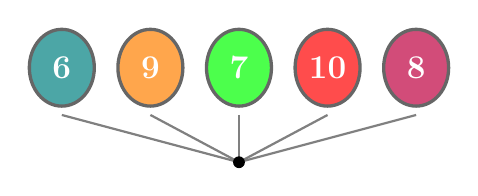
\begin{tikzpicture}[scale=0.75, baseline=(current bounding box.center)]
  \foreach \x/\num/\c in {-3/6/teal, -1.5/9/orange, 0/7/green, 1.5/10/red, 3/8/purple} {
    \draw[line width=0.8pt, gray] (\x,-0.8) -- (0,-1.6);
    \draw[fill=\c!70, draw=black!60, line width=1.2pt] (\x,0) ellipse (0.55cm and 0.65cm);
    \node[font=\large\bfseries, text=white] at (\x,0) {\num};
  }
  \fill[black] (0,-1.6) circle (0.1cm);
\end{tikzpicture}
\end{center}
\choice
{$9$}
{$8$}
{\True $10$}
{$7$}
\loigiai{
So sánh các số: $6 < 7 < 8 < 9 < 10$. Số lớn nhất là $10$.\\
\textbf{Đáp án của câu hỏi là C}
}
\end{ex}

% --- CÂU 9 ---
\begin{ex} %[1D1V02]
Trong các ngôi sao mang số $6, 8, 10, 7, 9$, ngôi sao nào mang số \textbf{bé nhất}?
\begin{center}
\begin{tikzpicture}[scale=0.75, baseline=(current bounding box.center)]
  \foreach \x/\num in {-3/8, -1.5/6, 0/10, 1.5/7, 3/9} {
    \node[draw=orange!80!black, fill=yellow!80, star, star points=5, star point ratio=2.2, line width=1.2pt, minimum size=1.1cm] at (\x,0) {};
    \node[font=\bfseries\normalsize, text=red!85!black] at (\x,-0.02) {\num};
  }
\end{tikzpicture}
\end{center}
\choice
{\True $6$}
{$7$}
{$8$}
{$9$}
\loigiai{
Trong các số $6, 8, 10, 7, 9$, số bé nhất là số $6$.\\
\textbf{Đáp án của câu hỏi là A}
}
\end{ex}

% --- CÂU 10 ---
\begin{ex} %[1D1V02]
Dãy thẻ số nào dưới đây được xếp đúng theo thứ tự từ bé đến lớn?
\begin{center}
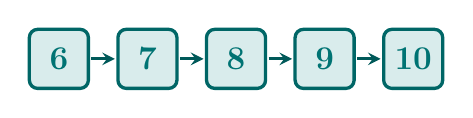
\begin{tikzpicture}[scale=0.75, baseline=(current bounding box.center)]
  \foreach \i/\num in {0/6, 1/7, 2/8, 3/9, 4/10} {
    \draw[fill=teal!15, draw=teal!80!black, line width=1.2pt, rounded corners=3pt] (\i*1.5,-0.4) rectangle (\i*1.5+1.0,0.6);
    \node[font=\large\bfseries, text=teal!90!black] at (\i*1.5+0.5, 0.1) {\num};
    \ifnum\i<4
      \draw[->, >=stealth, line width=1pt, teal!70!black] (\i*1.5+1.05,0.1) -- (\i*1.5+1.45,0.1);
    \fi
  }
\end{tikzpicture}
\end{center}
\choice
{$10, 9, 8, 7, 6$}
{\True $6, 7, 8, 9, 10$}
{$6, 8, 7, 9, 10$}
{$7, 6, 8, 9, 10$}
\loigiai{
Thứ tự đếm xuôi từ bé đến lớn: $6, 7, 8, 9, 10$.\\
\textbf{Đáp án của câu hỏi là B}
}
\end{ex}

% --- CÂU 11 ---
\begin{ex} %[1D1V02]
Có $6$ quả cam trong đĩa, mẹ để thêm $2$ quả cam nữa. Đếm tất cả có bao nhiêu quả cam?
\begin{center}
\begin{tikzpicture}[scale=0.7, baseline=(current bounding box.center)]
  % Đĩa cam có 6 quả
  \draw[fill=orange!10, draw=orange!70!black, line width=1.2pt] (-2.5,-0.2) ellipse (2.2cm and 0.7cm);
  \foreach \x/\y in {-3.5/0, -2.9/0.2, -2.3/0, -1.7/0.2, -2.0/-0.2, -2.8/-0.2} {
    \fill[orange!90!black] (\x,\y) circle (0.3cm);
    \fill[green!70!black] (\x,\y+0.3) circle (0.07cm);
  }
  \node[font=\small\bfseries] at (-2.5,-0.8) {6 quả};
  \node[font=\Large\bfseries, text=red] at (0,0.2) {$+$};
  % 2 quả ngoài đĩa
  \foreach \x in {1.8, 2.8} {
    \fill[orange!90!black] (\x,0) circle (0.3cm);
    \fill[green!70!black] (\x,0.3) circle (0.07cm);
  }
  \node[font=\small\bfseries] at (2.3,-0.8) {2 quả};
\end{tikzpicture}
\end{center}
\choice
{$7$ quả}
{\True $8$ quả}
{$9$ quả}
{$10$ quả}
\loigiai{
Đếm tất cả số quả cam: $6 + 2 = 8$ quả cam.\\
\textbf{Đáp án của câu hỏi là B}
}
\end{ex}

% --- CÂU 12 ---
\begin{ex} %[1D1C02]
Đếm số bạn bướm bay theo hàng từ số $6$ đến số $10$. Có tất cả bao nhiêu bạn bướm?
\begin{center}
\begin{tikzpicture}[scale=0.65, baseline=(current bounding box.center)]
  \foreach \i/\num in {0/6, 1/7, 2/8, 3/9, 4/10} {
    \begin{scope}[shift={(\i*2.2, 0.4)}, scale=0.45]
      \fill[magenta!70!purple] (-0.2,0.2) ellipse (0.4 and 0.6);
      \fill[magenta!70!purple] (0.2,0.2) ellipse (0.4 and 0.6);
      \fill[yellow!90!orange] (-0.2,-0.3) ellipse (0.3 and 0.4);
      \fill[yellow!90!orange] (0.2,-0.3) ellipse (0.3 and 0.4);
      \fill[black] (0,0) ellipse (0.1 and 0.5);
    \end{scope}
    \node[font=\bfseries\normalsize, text=blue!90!black] at (\i*2.2, -0.4) {Số \num};
  }
\end{tikzpicture}
\end{center}
\choice
{$4$ số}
{$6$ số}
{$7$ số}
{\True $5$ số}
\loigiai{
Có 5 số từ 6 đến 10: $6, 7, 8, 9, 10$.\\
Tương ứng với $5$ bạn bướm.\\
\textbf{Đáp án của câu hỏi là D}
}
\end{ex}

% =========================================================================
% PHẦN 2: TRẮC NGHIỆM ĐÚNG SAI (QUAN SÁT TRANH MINH HỌA)
% =========================================================================
\textbf{Phần 2. Trắc nghiệm đúng sai (Quan sát tia số và xét tính đúng/sai)}
\setcounterpageref{ex}{0}

% --- CÂU 13 ---
\begin{ex} %[1D1H02]
Quan sát tia số các bước nhảy từ $6$ đến $10$:
\begin{center}
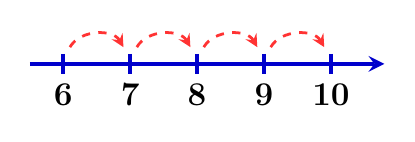
\begin{tikzpicture}[scale=0.85, baseline=(current bounding box.center)]
  \draw[->, >=stealth, line width=1.5pt, blue!80!black] (5.5,0) -- (10.8,0);
  \foreach \x in {6,7,8,9,10} {
    \draw[line width=1.5pt, blue!80!black] (\x,0.15) -- (\x,-0.15);
    \node[font=\bfseries\large, below] at (\x,-0.15) {\x};
  }
  \foreach \x in {6,7,8,9} {
    \draw[->, >=stealth, dashed, line width=1pt, red!80] (\x+0.1,0.25) to[out=60,in=120] (\x+0.9,0.25);
  }
\end{tikzpicture}
\end{center}
Xét tính đúng sai của các câu sau:
\choiceTF
{\True Số $10$ là số bé nhất có hai chữ số.}
{\True Số liền trước của số $8$ là số $7$.}
{Số liền sau của số $9$ là số $8$.}
{\True Số liền sau của số $9$ là số $10$.}
\loigiai{
\begin{itemize}
    \item Số $10$ là số bé nhất có hai chữ số: \textbf{Đúng}.
    \item Số $7$ đứng trước số $8$: \textbf{Đúng}.
    \item Số liền sau của số $9$ phải là $10$ (không phải $8$): \textbf{Sai}.
    \item Số liền sau của số $9$ là số $10$: \textbf{Đúng}.
\end{itemize}
}
\end{ex}

% --- CÂU 14 ---
\begin{ex} %[1D1V02]
Quan sát thứ tự dãy số từ $6$ đến $10$:
\begin{center}

\begin{tikzpicture}[scale=0.75, baseline=(current bounding box.center)]
  \foreach \i/\num/\c in {0/6/orange, 1/7/teal, 2/8/purple, 3/9/blue, 4/10/red} {
    \draw[fill=\c!20, draw=\c, line width=1.3pt, rounded corners=4pt] (\i*1.8,-0.4) rectangle (\i*1.8+1.3,0.8);
    \node[font=\LARGE\bfseries, text=\c!90!black] at (\i*1.8+0.65, 0.2) {\num};
  }
\end{tikzpicture}
\end{center}
Xét tính đúng sai của các câu sau:
\choiceTF
{\True Dãy số được sắp xếp theo thứ tự tăng dần.}
{\True Số đứng đầu dãy là $6$, số đứng cuối dãy là $10$.}
{Số $8$ đứng liền sau số $9$.}
{\True Số $8$ đứng liền trước số $9$.}
\loigiai{
\begin{itemize}
    \item Dãy số tăng dần: \textbf{Đúng}.
    \item Đầu dãy là $6$, cuối dãy là $10$: \textbf{Đúng}.
    \item Số $8$ đứng trước số $9$: \textbf{Sai} (câu c bảo đứng sau).
    \item Số $8$ đứng liền trước số $9$: \textbf{Đúng}.
\end{itemize}
}
\end{ex}

% =========================================================================
% PHẦN 3: TRẢ LỜI NGẮN (ĐIỀN SỐ THÍCH HỢP VÀO Ô TRỐNG)
% =========================================================================
\textbf{Phần 3. Trả lời ngắn (Quan sát hình vẽ và điền số thích hợp)}
\setcounterpageref{ex}{0}

% --- CÂU 15 ---
\begin{ex} %[1D1H02]
Đếm tổng số ngón tay trên cả hai bàn tay dưới đây:
\begin{center}

\begin{tikzpicture}[scale=0.6, baseline=(current bounding box.center)]
  \begin{scope}[shift={(-2,0)}]
    \draw[fill=yellow!30, draw=orange!85!black, line width=1.2pt]
      (0,-0.5) -- (-0.1,0.4) -- (-0.7,0.2) -- (-0.8,0.5) -- (-0.2,0.8)
      -- (-0.3,1.5) -- (0,1.5) -- (0.05,0.9)
      -- (0.08,1.7) -- (0.4,1.7) -- (0.42,0.9)
      -- (0.45,1.5) -- (0.75,1.5) -- (0.75,0.8)
      -- (0.78,1.2) -- (1.05,1.2) -- (1.0,0.3)
      -- (0.8,-0.5) -- cycle;
  \end{scope}
  \begin{scope}[shift={(2,0)}, xscale=-1]
    \draw[fill=yellow!30, draw=orange!85!black, line width=1.2pt]
      (0,-0.5) -- (-0.1,0.4) -- (-0.7,0.2) -- (-0.8,0.5) -- (-0.2,0.8)
      -- (-0.3,1.5) -- (0,1.5) -- (0.05,0.9)
      -- (0.08,1.7) -- (0.4,1.7) -- (0.42,0.9)
      -- (0.45,1.5) -- (0.75,1.5) -- (0.75,0.8)
      -- (0.78,1.2) -- (1.05,1.2) -- (1.0,0.3)
      -- (0.8,-0.5) -- cycle;
  \end{scope}
\end{tikzpicture}
\end{center}
\shortans{10}
\loigiai{
\textbf{Đáp số:} $10$\\
Hai bàn tay có tất cả $10$ ngón tay.
}
\end{ex}

% --- CÂU 16 ---
\begin{ex} %[1D1H02]
Điền số liền sau của số $7$ vào ô trống còn thiếu:
\begin{center}
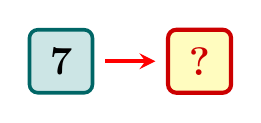
\begin{tikzpicture}[scale=0.8, baseline=(current bounding box.center)]
  \draw[fill=teal!20, draw=teal!80!black, line width=1.3pt, rounded corners=3pt] (-1.2,-0.4) rectangle (-0.2,0.6);
  \node[font=\Large\bfseries] at (-0.7,0.1) {7};
  \draw[->, >=stealth, line width=1.5pt, red] (0,0.1) -- (0.8,0.1);
  \draw[fill=yellow!25, draw=red!80!black, line width=1.5pt, rounded corners=3pt] (1.0,-0.4) rectangle (2.0,0.6);
  \node[font=\Large\bfseries, text=red!80!black] at (1.5,0.1) {?};
\end{tikzpicture}
\end{center}
\shortans{8}
\loigiai{
\textbf{Đáp số:} $8$\\
Số liền sau của số $7$ là số $8$.
}
\end{ex}

% --- CÂU 17 ---
\begin{ex} %[1D1V02]
Điền số liền trước của số $10$ vào ô trống còn thiếu:
\begin{center}
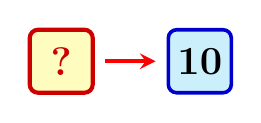
\begin{tikzpicture}[scale=0.8, baseline=(current bounding box.center)]
  \draw[fill=yellow!25, draw=red!80!black, line width=1.5pt, rounded corners=3pt] (-1.5,-0.4) rectangle (-0.5,0.6);
  \node[font=\Large\bfseries, text=red!80!black] at (-1.0,0.1) {?};
  \draw[->, >=stealth, line width=1.5pt, red] (-0.3,0.1) -- (0.5,0.1);
  \draw[fill=cyan!20, draw=blue!80!black, line width=1.3pt, rounded corners=3pt] (0.7,-0.4) rectangle (1.7,0.6);
  \node[font=\Large\bfseries] at (1.2,0.1) {10};
\end{tikzpicture}
\end{center}
\shortans{9}
\loigiai{
\textbf{Đáp số:} $9$\\
Số liền trước của số $10$ là số $9$.
}
\end{ex}

% --- CÂU 18 ---
\begin{ex} %[1D1V02]
Số nào đứng ở giữa số $6$ và số $8$?
\begin{center}
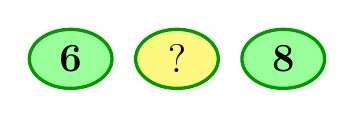
\begin{tikzpicture}[scale=0.75, baseline=(current bounding box.center)]
  \foreach \x/\num/\c in {-1.8/6/green!40, 0/{$\mathbf{?}$}/yellow!50, 1.8/8/green!40} {
    \draw[fill=\c, draw=green!60!black, line width=1.2pt] (\x,0) ellipse (0.7cm and 0.5cm);
    \node[font=\Large\bfseries] at (\x,0) {\num};
  }
\end{tikzpicture}
\end{center}
\shortans{7}
\loigiai{
\textbf{Đáp số:} $7$\\
Số đứng giữa $6$ và $8$ là số $7$.
}
\end{ex}

% --- CÂU 19 ---
\begin{ex} %[1D1V02]
Trong bể có $5$ con cá vàng, thả thêm $4$ con cá xanh. Hỏi trong bể có tất cả bao nhiêu con cá?
\begin{center}
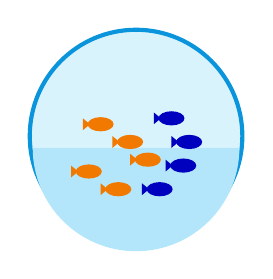
\begin{tikzpicture}[scale=0.75, baseline=(current bounding box.center)]
  \draw[fill=cyan!15, draw=cyan!80!blue, line width=1.5pt] (0,0) circle (1.8cm);
  \fill[cyan!30] (-1.75,-0.2) arc (180:360:1.75cm) -- cycle;
  % 5 cá vàng
  \foreach \px/\py in {-0.8/-0.6, -0.3/-0.9, -0.6/0.2, 0.2/-0.4, -0.1/-0.1} {
    \fill[orange!95!black] (\px,\py) ellipse (0.22cm and 0.12cm);
    \fill[orange!95!black] (\px-0.18,\py) -- (\px-0.3,\py+0.1) -- (\px-0.3,\py-0.1) -- cycle;
  }
  % 4 cá xanh
  \foreach \px/\py in {0.6/0.3, 0.8/-0.5, 0.4/-0.9, 0.9/-0.1} {
    \fill[blue!75!black] (\px,\py) ellipse (0.22cm and 0.12cm);
    \fill[blue!75!black] (\px-0.18,\py) -- (\px-0.3,\py+0.1) -- (\px-0.3,\py-0.1) -- cycle;
  }
\end{tikzpicture}
\end{center}
\shortans{9}
\loigiai{
\textbf{Đáp số:} $9$\\
Trong bể có tất cả $5 + 4 = 9$ con cá.
}
\end{ex}

% --- CÂU 20 ---
\begin{ex} %[1D1C02]
Đếm số ngôi sao mang số có \textbf{một chữ số lớn hơn 5} dưới đây:
\begin{center}
\begin{tikzpicture}[scale=0.75, baseline=(current bounding box.center)]
  \foreach \i/\num in {0/6, 1/7, 2/8, 3/9} {
    \node[draw=orange!80!black, fill=yellow!85, star, star points=5, star point ratio=2.2, line width=1.2pt, minimum size=1.1cm] at (\i*1.6,0) {};
    \node[font=\bfseries\normalsize, text=red!85!black] at (\i*1.6,-0.02) {\num};
  }
\end{tikzpicture}
\end{center}
\shortans{4}
\loigiai{
\textbf{Đáp số:} $4$\\
Có $4$ số có một chữ số lớn hơn $5$ là: $6, 7, 8, 9$.
}
\end{ex}
